\section{Query Algorithms}
\label{query}

In this section, we present three query algorithms based on the CL-tree index.
Based on how we verify the candidate keyword sets, we divide our algorithms into incremental algorithms (from examining smaller candidate sets to larger ones) and decremental algorithm (from examining larger candidate sets to smaller ones).
We propose two incremental algorithms called \textbf{{\tt Inc-S}} (\underline{Inc}remental \underline{S}pace efficient) and \textbf{{\tt Inc-T}} (\underline{Inc}remental \underline{T}ime efficient), to trade off between the memory consumption and the computational overhead.
The decremental algorithm is called \textbf{{\tt Dec}} (\underline{Dec}remental).
Our interesting finding is that, while {\tt Dec} seems not intuitive, it ranks as the most efficient one.
{\tt Inc-S} and {\tt Inc-T} are presented in Section~\ref{inc}.
{\tt Dec} is introduced in Section~\ref{dec}.

\subsection{The Incremental Algorithms}
\label{inc}

While the high-level idea of incremental algorithms resembles the basic solutions (see Section~\ref{basic}),
{\tt Inc-S} and {\tt Inc-T} advance them with the exploitation of the CL-tree.
Specifically, they can always verify the existence of $G_k[S']$ within a subgraph of $G$ instead of the entire graph $G$. More interestingly, the subgraph for such verifications shrinks when the candidate set $S'$ expands. Therefore, a large sum of redundant computation is cut off during the verification. We present {\tt Inc-S} and {\tt Inc-T} in Sections~\ref{inc-S} and~\ref{inc-T}.


\subsubsection{Inc-S Algorithm}
\label{inc-S}
We first introduce a new concept, called \textbf{subgraph core number},
which is geared to the main idea of {\tt Inc-S}.

\begin{definition}[Subgraph core number]
\label{def:ccscore}
  The core number of a subgraph $G'$ of $G$, $core_G[G']$,
  is defined as $min\{core_G[v]|$ $v\in G'\}$.
\end{definition}


{\tt Inc-S} follows the two-step framework (\emph{verification} and \emph{candidate generation})
introduced in Section~\ref{basic}. With the CL-tree, we improve the verification step as follows.
\begin{itemize}
\item {\bf Core-based verification.} For each newly generated size-($c$+1) candidate keyword set $S'$ expanded from size-$c$ sets $S_1$ and $S_2$, mark $S'$ as a qualified set if $G_k[S']$ exists \textit{in a subgraph of core number} $max\{core_G[G_k[S_1]]$, $core_G[G_k[S_2]]\}$.
\end{itemize}

The core-based verification guarantees that, with the expansion of the candidate keyword sets, the verification becomes faster as it only needs to examine the existence of $G_k[S']$ in a smaller $k$-$\widehat {core}$ (Recall that cores with large core numbers are nested in the cores with small core numbers). The correctness of such shrunk verification range is guaranteed by the following lemma.
\begin{lemma}
\label{lemma:coreDown}
  Given two subgraphs $G_k[S_1]$ and $G_k[S_2]$ of a graph $G$,
  for a new keyword set $S'$ generated from $S_1$ and $S_2$ (\textit{i.e.}, $S'=S_1\cup S_2$),
  if $G_k[S']$ exists, then it must appear in a $k$-$\widehat {core}$ with core number at least
  \begin{equation}
    max\{core_G[G_k[S_1]], core_G[G_k[S_2]]\}.
  \end{equation}
\end{lemma}

The verification process can be further accelerated by checking the numbers of vertices and edges,
as indicated by Lemma~\ref{lemma:coreExist}.
\begin{lemma}
\label{lemma:coreExist}
  Given a connected graph $G(V,E)$ with $n$=$|V|$ and $m$=$|E|$,
  if $m - n < \frac{{{k^2} - k}}{2} - 1$, there is no $k$-$\widehat {core}$ in $G$.
\end{lemma}

This lemma implies that, for a connected subgraph $G'$, whose edge and vertex numbers are $m$ and $n$,
if $m - n < \frac{{{k^2} - k}}{2} - 1$, then we cannot find $G_k[S']$ from $G'$.

We present {\tt Inc-S} in Algorithm~\ref{alg:incS}.
The input is a CL-tree rooted at $root$, a query vertex $q$, a positive integer $k$ and a keyword set $S$.
We apply {\tt core-locating} on the CL-tree to locate the internal nodes whose corresponding $k$-$\widehat {core}$s contain $q$ (line 2).
Note that their core numbers are in the range of $[k,core_G[q]]$, as required by the structure cohesiveness.
Then, we set $l$=0, indicating the sizes of current keyword sets, and initialize a set $\Psi$ of $\textless S',c\textgreater$ pairs,
where $S'$ is a set containing a keyword from $S$ and $c$ is the initial core number $k$ (line 3).
Note that we skip those keywords, which are in $S$, but not in $W(q)$.
In the while loop (lines 4-18), for each $\textless S',c\textgreater$ pair,
we first perform {\tt keyword-checking} to find $G[S']$ using the keyword inverted lists of the subtree rooted at node $r_c$.
If we cannot ensure that $G[S']$ does not contain a $k$-$\widehat {core}$ by Lemma~\ref{lemma:coreExist},
we then find $G_k[S']$ from $G[S']$ (lines 8-9).
If $G_k[S']$ exists, we put $S'$ with its core number into the set $\Phi_l$ (lines 10-11).
Next, if $\Phi_l$ is nonempty, we generate new candidates by calling \textsc{geneCand($\Phi_{l}$)},
which is detailed in Appendix~\ref{app:geneCand}.
For each candidate $S'$ in $\Psi$, we compute the core number using Lemma~\ref{lemma:coreDown}
and update it as a pair in $\Psi$ (lines 12-17);
otherwise, we stop (line 18).
Finally, we output the communities of the latest verified keyword sets (line 19).

\begin{algorithm}[h]
\caption{Query algorithm: {\tt Inc-S}}
\label{alg:incS}
\footnotesize{
\algrenewcommand{\algorithmiccomment}[1]{\hskip3em$//$ #1}
\begin{algorithmic}[1]
    \Function{query($G$, $root$, $q$, $k$, $S$)}{}
        \State find subtree root nodes $r_k,r_{k+1},\cdots,r_{core_G[q]}$;
        \State initialize $l$=0, $\Psi$ using $S$;
        \While{$true$}
            \State $l\gets l+1$; $\Phi_{l} \gets \emptyset$;
            \For {each $\textless S',c \textgreater$ $\in \Psi$}
                \State find $G[S']$ under the root $r_c$;
                \If {$G[S']$ is not pruned by Lemma~\ref{lemma:coreExist}}
                    \State find $G_k[S']$ from $G[S']$;
                    \If {$G_k[S']$ exists}
                        \State $\Phi_{l}$.add($\textless S', core_G[G_k[S']]\textgreater$);
                    \EndIf
                \EndIf
            \EndFor

            \If{$\Phi_{l} \ne \emptyset$}
                \State $\Psi \gets$ \Call{geneCand($\Phi_{l}$)}{};
                \For {each $S'$ in $\Psi$}
                    \If {$S'$ is generated from $S_1$ and $S_2$}
                        \State $c\gets max\{core_G[G_k[S_1]],core_G[G_k[S_2]]\}$;
                        \State $\Psi$.update($S'$, $\textless S',c\textgreater$);
                    \EndIf
                \EndFor
            \Else {} break;
            \EndIf
        \EndWhile
        \State output the communities of keyword sets in $\Phi_{l-1}$;
    \EndFunction
\end{algorithmic}}
\end{algorithm}

\begin{example}
\label{eg:inc-S}
Consider the graph in Figure~\ref{fig:kcoreGraph}
and its index in Figure~\ref{fig:cktree}.
Let $q$=$A$, $k$=1 and $S$=$\{w,x,y\}$.
By Algorithm~\ref{alg:incS}, we first find 3 root nodes $r_1$, $r_2$ and $r_3$.
In the first while loop, we find 2 qualified keyword sets $\{x\}and \{y\}$ with core numbers being 3 and 1.
By Lemma~\ref{lemma:coreDown}, we only need to verify the new candidate keyword set $\{x,y\}$ under node $r_3$.
\end{example}

\subsubsection{Inc-T Algorithm}
\label{inc-T}
We begin with a lemma which inspires the design of {\tt Inc-T}.
\begin{lemma}
\label{lemma:kcoreIntersect}
  Given two keyword sets $S_1$ and $S_2$, if $G_k[S_1]$ and $G_k[S_2]$ exist, we have
  \begin{equation}
    %{G_k}[{S_1} \cup {S_2},q] \subseteq {G_k}[{S_1},q] \cap {G_k}[{S_2},q].
    G_k[S_1\cup S_2] \subseteq G_k[S_1]\cap G_k[S_2].
  \end{equation}
\end{lemma}

This lemma implies, if $S'$ is generated from $S_1$ and $S_2$,
we can find $G_k[S']$ from $G_k[S_1]\cap G_k[S_2]$ directly.
Since every vertex in $G_k[S_1]\cap G_k[S_2]$ contains both $S_1$ and $S_2$,
we do not need to consider the keyword constraint again when finding $G_k[S']$.

Based on Lemma~\ref{lemma:kcoreIntersect}, we introduce a new algorithm \textbf{{\tt Inc-T}}. Different from {\tt Inc-S}, {\tt Inc-T} maintains $G_k[S']$ rather than $core_G[$ $G_k[S']]$ for each qualified keyword set $S'$. As we will demonstrate later, {\tt Inc-T} is more effective for shrinking the subgraphs containing the ACs, and thus more efficient. As a trade-off for better efficiency, {\tt Inc-T} consumes more memory as it needs to store a list of subgraph $G_k[S']$ in memory.

\begin{algorithm}[h]
\caption{Query algorithm: {\tt Inc-T}}
\label{alg:incT}
\footnotesize{
\algrenewcommand{\algorithmiccomment}[1]{\hskip3em$//$ #1}
\begin{algorithmic}[1]
    \Function{query($G$, $root$, $q$, $k$, $S$)}{}
        \State find the $k$-$\widehat {core}$, which contains $q$;
        \State initialize $l$=0, $\Psi$ using $S$;
        \While{$true$}
            \State $l\gets l+1$; $\Phi_{l} \gets \emptyset$;
            \For {each $<S',\widehat{G}>$ $\in \Psi$}
                \State find $G[S']$ from $\widehat{G}$;
                \If {$G[S']$ is not pruned by Lemma~\ref{lemma:coreExist}}
                    \State find $G_k[S']$ from $G[S']$;
                    \If {$G_k[S']$ exists}
                        \State $\Phi_{l}$.add($<S', G_k[S']>$);
                    \EndIf
                \EndIf
            \EndFor
            \If {$\Phi_{l} \ne \emptyset$}
                \State $\Psi \gets$ \Call{geneCand($\Phi_{l}$)}{};
                \For {each $S' \in \Psi$}
                    \If {$S'$ is generated from $S_1$ and $S_2$}
                        \State $\widehat G \gets G_k[S_1]\cap G_k[S_2]$;
                        \State $\Psi_{l}$.update($S'$,$<S',\widehat G>$);
                   \EndIf
                \EndFor
            \Else {} break;
            \EndIf
        \EndWhile
        \State output the communities of keyword sets in $\Phi_{l-1}$;
    \EndFunction
\end{algorithmic}}
\end{algorithm}

Algorithm~\ref{alg:incT} presents the steps of {\tt Inc-T}.
We first apply {\tt core-locating} to find the $k$-$\widehat{core}$ containing $q$ from the CL-tree (line 2).
Then, we set $l$=0, indicating the sizes of current keyword sets,
and initialize a set $\Psi$ of $<S',\widehat G>$ pairs,
where $S'$ is a set containing a keyword from $S$ and $\widehat G$ is the $k$-$\widehat {core}$.
The while loop (lines 4-18) is similar with that of {\tt Inc-S}.
The main differences are that:
(1) for each qualified keyword set $S'$, {\tt Inc-T} keeps $G_k[S']$ in memory (line 11);
and (2) for each candidate keyword set $S'$ generated from $S_1$ and $S_2$,
{\tt Inc-T} finds $G_k[S']$ from $G_k[S_1]\cap G_k[S_2]$ directly without further keyword verification (lines 6-9, 16).

\begin{example}
\label{eg:inc-T}
Continue the graph and query ($q$=$A$, $k$=1, $S$=$\{w$, $x,y\}$) in Example~\ref{eg:inc-S}.
By {\tt Inc-T}, we first find $G_1[\{x\}]$ and $G_1[\{y\}]$,
whose vertex sets are $\{A,B,C,D\}$ and $\{A,C,D$, $E,F,G\}$.
Then to find $G_1[\{x,y\}]$, we only need to search it from the subgraph,
induced by the vertex set $\{A,C,D\}$.
\end{example}




\subsection{The Decremental Algorithm}
\label{dec}

The decremental algorithm, denoted by {\tt Dec}, differs from previous query algorithms
not only on the generation of candidate keyword sets,
but also on the verification of candidate keyword sets.

\textbf{1. Generation of candidate keyword sets.}
{\tt Dec} exploits the key observation that,
if $S'$ ($S'\subseteq S$) is a qualified keyword set,
then there are at least $k$ of $q$'s neighbors containing set $S'$.
This is because every vertex in $G_k[S']$ must has degree at least $k$.
This observation implies,
we can generate all the candidate keyword sets directly by using the query vertex $q$ and $q$'s neighbors,
without touching other vertices.

Specifically, we consider $q$ and $q$'s neighbor vertices.
For each vertex $v$, we only select the keywords, which are contained by $S$ and at least $k$ of its neighbors.
Then we use these selected keywords to form an itemset, in which each item is a keyword.
After this step, we obtain a list of itemsets.
Then we apply the well studied frequent pattern mining algorithms
(e.g., Apriori~\cite{han2011data} and FP-Growth~\cite{han2000mining})
to find the frequent keyword combinations,
each of which is a candidate keyword set.
Since our goal is to generate keyword combinations shared by at least $k$ neighbors,
we set the minimum support as $k$.
In this paper, we use the well-known FP-Growth algorithm~\cite{han2000mining}.

\begin{figure}[ht]
    \centering
    \mbox{
        \subfigure[a query vertex]{
            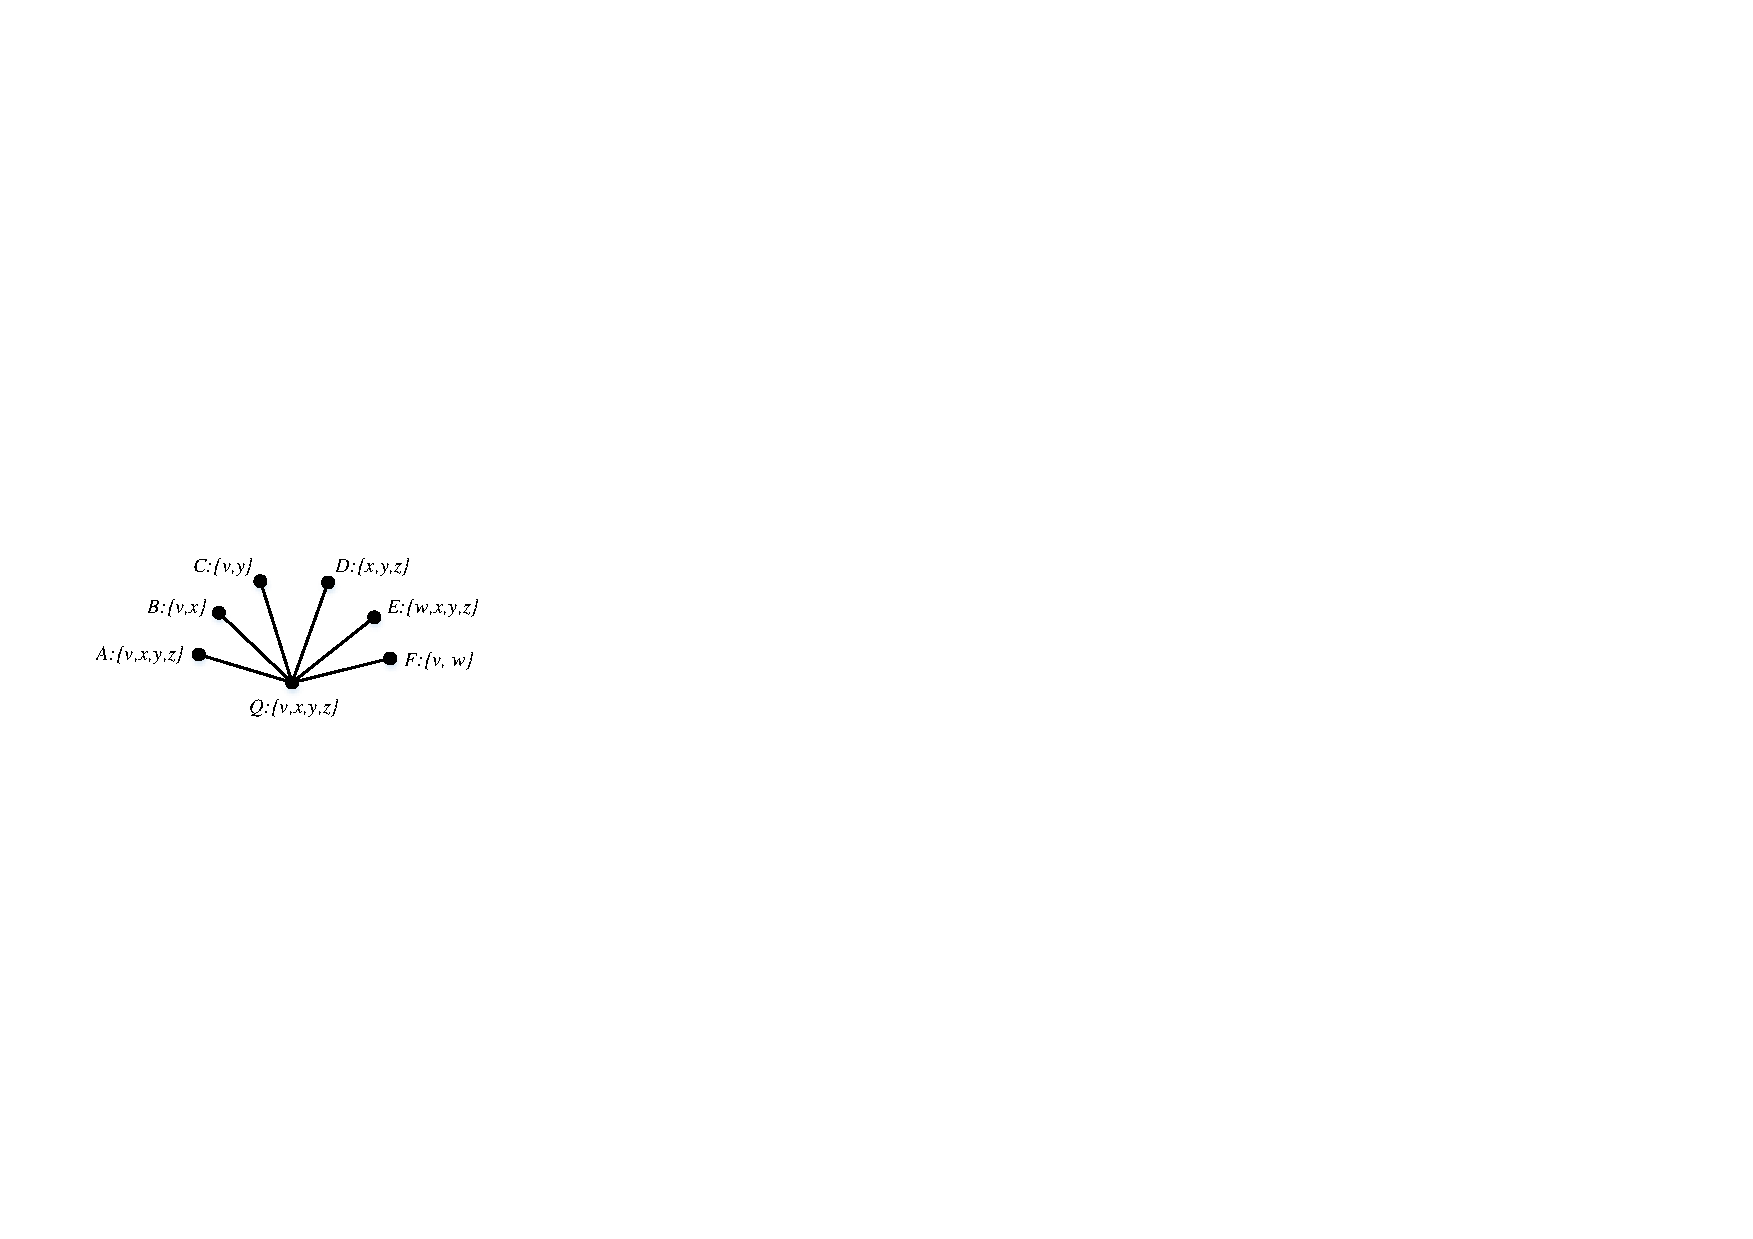
\includegraphics[width=.51\columnwidth]{figures/nghGraph}
            \label{fig:nghGraph}
        }
        \hspace{1ex}
        \subfigure[candidates]{
            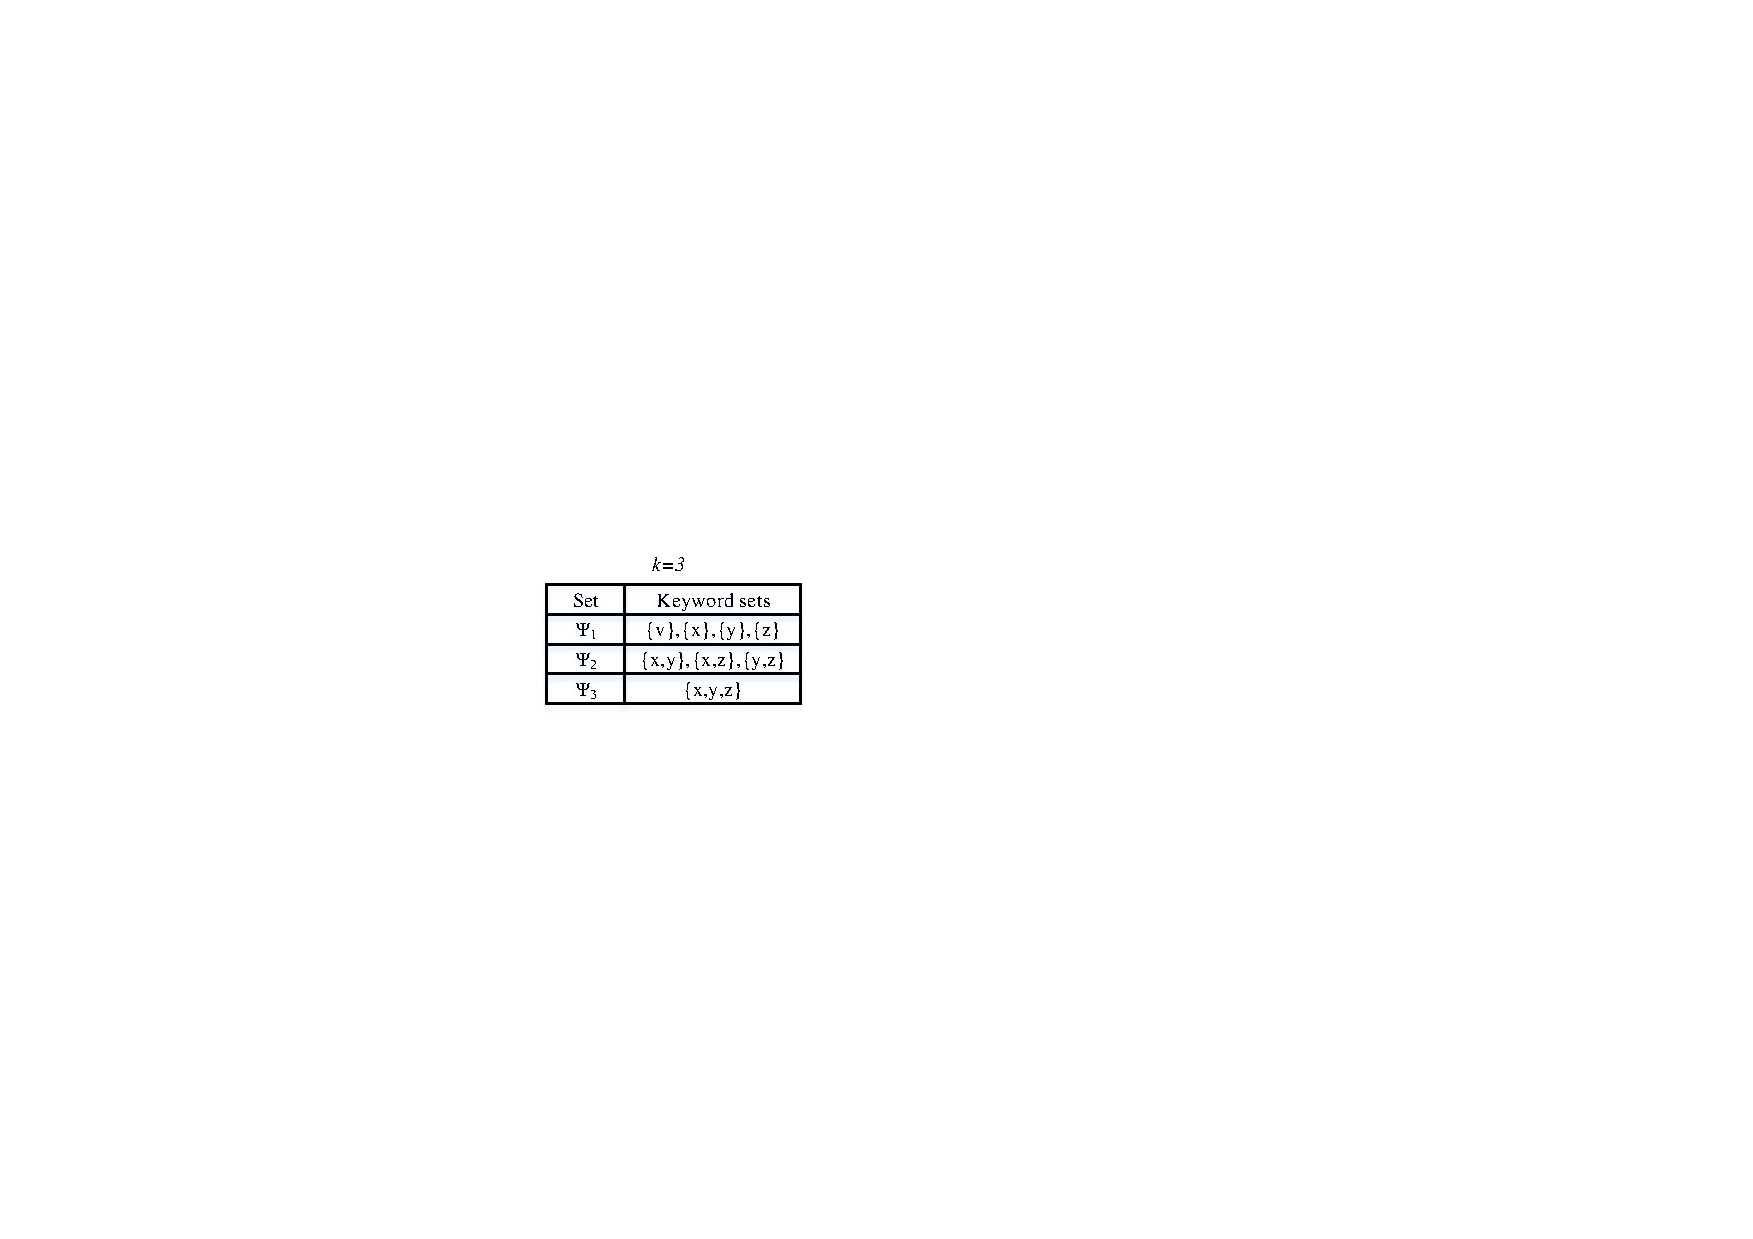
\includegraphics[width=.34\columnwidth]{figures/nghCand}
            \label{fig:nghCand}
        }
    }
    \caption{An example of candidate generation.}
\end{figure}
\begin{example}
Consider a query vertex $Q$ ($k$=3, $S$=$\{v,x,y,z\}$) with 6 neighbors in Figure~\ref{fig:nghGraph},
where the selected keywords of each vertex are listed in the curly braces.
By FP-Growth, 8 candidate keyword sets) are generated, as shown in Figure~\ref{fig:nghCand}.
$\Psi_i$ denotes the set of keyword sets with sizes being $i$.
\end{example}

\textbf{2. Verification of candidate keyword sets.}
As candidates can be obtained using $S$ and $q$'s neighbors directly,
we can verify them either incrementally as that in {\tt Inc-S},
or in a decremental manner (larger candidate keyword sets first and smaller candidate keyword sets later).
In this paper, we choose the latter manner. The rationale behind is that,
for any two keyword sets $S_1\subseteq S_2$, the number of vertices containing $S_2$ is usually smaller than that of $S_1$,
which implies $S_2$ can be verified more efficiently than $S_1$.

\begin{algorithm}[h]
\caption{Query algorithm: {\tt Dec}}
\label{alg:ngh}
\footnotesize{
\algrenewcommand{\algorithmiccomment}[1]{\hskip3em$//$ #1}
\begin{algorithmic}[1]
    \Function{query($G$, $root$, $q$, $k$, $S$)}{}
        \State generate $\Psi_1,\Psi_2,\cdots, \Psi_h$ using $S$ and $q$'s neighbors;
        \State find the subtree root node $r_k$;
        \State create $R_1,R_2,\cdots,R_{h'}$ by using subtree rooted at $r_k$;
        \State $l\gets h$; $Q\gets \emptyset$;
        \State ${\widehat R}\gets {R_h} \cup \cdots \cup {R_{h'}}$;
        \While {$l\geq 1$}
            \For {each $S'\in \Psi_l$}
                \State find $G[S']$ from the subgraph induced on $\widehat R$;
                \State find $G_k[S']$ from $G[S']$;
                \If {$G_k[S']$ exists}
                    $Q$.add($G_k[S']$);
                \EndIf
            \EndFor
            \If {$Q$=$\emptyset$}
                \State $l\gets l-1$;
                \State ${\widehat R}\gets {\widehat R}\cup R_l$;
            \Else {} break;
            \EndIf
        \EndWhile
        \State output communities in $Q$;
    \EndFunction
\end{algorithmic}}
\end{algorithm}

Based on the above discussions, we design {\tt Dec} as shown in Algorithm~\ref{alg:ngh}.
We first generate candidate keyword sets using $S$ and $q$'s neighbors by FP-Growth algorithm (line 2).
Then, we apply {\tt core-locating} to find the root (with core number $k$) of the subtree from CL-tree,
whose corresponding $k$-$\widehat {core}$ contains $q$ (line 3).
Next, we traverse the subtree rooted at $r_k$
and find vertices which share keywords with $q$ (line 4).
$R_i$ denote the sets of vertices sharing $i$ keywords with $q$.
Then, we initialize $l$ as $h$ (line 5),
as we verify keyword sets with the largest size $h$ first.
We maintain a set $\widehat R$ dynamically,
which contains vertices sharing at least $l$ keywords with $q$ (line 6).
In the while loop, we examine candidate keyword sets in the decremental manner.
For each candidate $S'\in\Psi_l$, we first try to find $G[S']$, then find $G_k[S']$,
and put $G_k[S']$ into $Q$ if it exists (lines 8-11).
Finally, if we have found at least one qualified community,
we stop at the end of this loop and output $Q$;
otherwise, we examine smaller candidate keyword sets in next loop.  